\documentclass[11pt]{article}
\usepackage[utf8]{inputenc}
\usepackage{geometry}
\usepackage{graphicx}
\usepackage{titlesec}
\usepackage{fancyhdr}
\usepackage{listings} 
\usepackage{xcolor} 
\usepackage[colorlinks=true, linkcolor=black, urlcolor=blue, citecolor=black]{hyperref}
\usepackage{setspace}
\usepackage{datetime}

\geometry{margin=1in}
\setstretch{1.25}
\pagestyle{fancy}
\fancyhf{}
\rhead{\thepage}
\lhead{Mini Project 2: PirateEase Chatbot}

% Configure listings for Python code
\lstset{
    language=Python,
    basicstyle=\ttfamily\small,
    keywordstyle=\color{blue},
    stringstyle=\color{red},
    commentstyle=\color{green!50!black},
    showstringspaces=false,
    breaklines=true,
    numbers=left,
    numberstyle=\tiny\color{gray},
    frame=single,
    rulecolor=\color{black!30},
    tabsize=4,
    captionpos=b
}

% Cover Page Command
\newcommand{\coverpage}{
    \begin{titlepage}
        \centering
        \vspace*{3cm}
        {\Huge\bfseries Mini Project 2 \\ PirateEase Chatbot\par}
        \vspace{2cm}
        {\Large\itshape Brysen Pfingsten\par}
        \vfill
        {\large \today\par}
        \vspace{1cm}
        {\large Dr. Shajina Anand, CSAS 2124, Seton Hall University\par}
        \vspace*{2cm}
    \end{titlepage}
}

\begin{document}

\coverpage

\tableofcontents
\newpage

\section{Introduction}
The focus of this project was to explore how object-oriented design patterns can be used to build a chatbot that is both dynamic in its interaction with users and easily extensible for future upgrades. The chatbot is designed to handle 40 predefined queries, along with at least 3 additional flexible queries. \\
\noindent
To achieve this, I applied object-oriented principles and design patterns to create a full-stack application. The frontend allows users to interact with the chatbot through the command line, while the backend is responsible for retrieving data from JSON files and generating dynamic responses. This approach gives the chatbot the feel of a real large language model (LLM) utilizing retrieval-augmented generation (RAG).

\section{Creational Design Patterns} 
\subsection{Singleton} 
The \texttt{Singleton} pattern is used extensively throughout this project to ensure that only one instance of a given class is created during the program's lifecycle. To streamline this process, I created a base Singleton class that other classes could inherit from. This class overrides the \texttt{\_\_new\_\_} method and stores instances in a shared dictionary, allowing for efficient and consistent access to single instances across the application.	
\begin{lstlisting}
class Singleton:
    # Dictionary mapping classes to their instances
    _instances: dict = {}

    def __new__(cls):
        if cls not in cls._instances:
            instance = super().__new__(cls)
            instance._initialized = False
            cls._instances[cls] = instance
        return cls._instances[cls]
\end{lstlisting}
%
\noindent
When applied to backend services, the \texttt{Singleton} pattern ensures consistent and synchronized data as the user interacts with PirateEase. For example, the \texttt{OrderService} class inherits from the \texttt{Singleton} base class and, upon its first and only initialization, loads JSON data from a file and structures it into a list of \texttt{Order} objects. This approach improves efficiency by reducing memory usage and load times, while guaranteeing that any updates to the order data are reflected consistently throughout the application. This pattern is applied uniformly across all backend services to maintain coherence and performance.
\begin{lstlisting}
class OrderService(Singleton):
    def __init__(self):
        # If already initialized, skip
        if self._initialized:
            return
        # Load orders from DB
        with open('Databases/orders.json', 'r', encoding='utf-8') as f:
            raw_orders: dict = json.load(f)
            self.__orders: dict[int, Order] = {
                int(order_id): Order(
                    id=int(order_id),
                    customer_name=data["customer_name"],
                    order_date=data["order_date"],
                    eta_hours=data["eta_hours"],
                    item=data["item"],
                    quantity=data["quantity"],
                    refunded=False
                )
                for order_id, data in raw_orders.items()
            }
        # Mark as initialized
        self._initialized = True

    def retrieve_order(self, order_id: str) -> str:
        # Get the order from the DB
        order: Order = self.__orders.get(int(order_id))
        if order is not None:  # If an order matched
            return str(order)  # Return its string representation
        else:  # No order matched the order ID
            return ''  # Return an empty string
\end{lstlisting}
%
Additionally, the \texttt{Singleton} pattern is applied to the \texttt{SessionManager} to ensure that its state and history remain consistent and accessible throughout the entire program. This allows the application to reliably track user interactions—such as appending to the session history or retrieving session state—while handling input in the \texttt{UserInterface} class and across all \texttt{QueryHandler} components.
%
\begin{lstlisting}
# In PirateEase.Utils.session_manager
class SessionManager(Singleton):
    def __init__(self):
        if self._initialized:
            return
        self.__state: dict[str, str] = {}
        self.__history: list[str] = []
        self._initialized = True
        
# In PirateEase.Utils.user_interface
class UserInterface:
	
	...	
	
    @classmethod
    def get_refund_reason(cls):
        message: str = 'PirateEase: ' + ResponseFactory.get_response('refund_reason')
        slow_print(message)
        cls.session.append_history(message)
        refund_reason: str = input('User: ').strip()
        cls.session.append_history(f'User: {refund_reason}')
        return refund_reason
        
# In PirateEase.Queries.order_tracking_handler
class OrderTrackingHandler(QueryHandler):
    def handle(self, query: str) -> str:
        if 'order_id' in self._session:
            order_id: str = self._session.get('order_id')
            return self._backend.process_request('order', order_id)

        order_id: str = UserInterface.get_order_id()
        response = self._backend.process_request('order', order_id)
        while not response:
            not_found_response: str = 'PirateEase: ' + ResponseFactory.get_response('order_not_found').format(order_id=order_id)
            self._session.append_history(not_found_response)
            slow_print(not_found_response)
            order_id = UserInterface.get_order_id()
            response = self._backend.process_request('order', order_id)

        self._session.set('order_id', order_id)
        return response
\end{lstlisting}
%
%
%
\subsection{Factory}
Another creational pattern used in this project is the \texttt{Factory} pattern. This pattern encapsulates the object creation logic, allowing for greater flexibility and decoupling in how new instances are constructed. A key example is the \texttt{ResponseFactory}, which is responsible for generating dynamic responses based on the specified query category. It also includes predefined response templates with runtime variable substitution, enabling more natural and context-aware replies.
\begin{lstlisting}
class ResponseFactory:
    with open('Databases/responses.json', 'r', encoding='utf-8') as f:
        responses: dict[str, list[str]] = json.load(f)

    @classmethod
    def get_response(cls, category: str) -> str:
        return random.choice(cls.responses[category])
\end{lstlisting}
%
Some examples of categories and responses are below.
%
\begin{lstlisting}
"product_available": [
    "{item} is in stock at {price}! Only {quantity} remaining.",
    "{item} can be yours today for {price}! We got {quantity} left.",
    "{item} is up for grabs at {price}! {quantity} available now.",
    "{item} is ready to ship for just {price}! Only {quantity} in stock.",
    "Good news! {item} is available for {price} - {quantity} left!",
    "Act fast! {quantity} units of {item} remaining at {price} each.",
    "Yes! {item} is here at {price}, with {quantity} in stock.",
    "Get your {item} now for {price}! Only {quantity} left.",
    "{item} just hit the shelves for {price}! {quantity} up for grabs."
  ],
  "not_available": [
    "{item} is currently out of stock.",
    "Sorry, we're fresh out of {item}.",
    "Looks like {item} is temporarily unavailable.",
    "Ahoy! {item} is all gone for now.",
    "No more {item} at the moment-check back soon!",
    "We have run out of {item}, unfortunately.",
    "{item} is out of commission for the time being.",
    "Heads up! {item} is not available right now."
  ]
\end{lstlisting}
%
Additionally, the \texttt{Factory} pattern is employed when dynamically retrieving \texttt{QueryHandler} instances based on intent types. The \texttt{QueryManager} class encapsulates a dictionary that maps intent strings to their corresponding \texttt{QueryHandler} classes. It exposes a \texttt{get\_handler()} interface, which returns the appropriate handler instance for a given intent, streamlining the routing of user queries to the correct logic.
\begin{lstlisting}
class QueryManager:
    def __init__(self):
        self.handlers: dict[str, QueryHandler] = {
            "order": OrderTrackingHandler(),
            "refund": RefundHandler(),
            "inventory": ProductAvailabilityHandler(),
            "live_agent": LiveAgentHandler(),
            "exit": ExitHandler(),
            "db": QueryDatabase(),
            "unknown": DefaultHandler()
        }

    def get_handler(self, query_type: str) -> QueryHandler:
        return self.handlers.get(query_type.lower())
\end{lstlisting}
%
\section{Structural Design Patterns}
\subsection{Facade}
%
The \texttt{Facade} pattern is used in this project to coordinate various subsystems and components through a simplified interface that abstracts away internal complexity. For example, the \texttt{ChatBot} class acts as a facade by managing interactions between session history, backend services, intent recognition, and the query manager—all through a single \texttt{process\_query()} interface.
%
\begin{lstlisting}
class ChatBot:
	
	...
	
    def process_query(self, query: str) -> str:
        # Add the query to the history
        self.__session_manager.append_history('User: ' + query)
        # Setup up global variables to be used later
        response: str = ''
        db_response: str = self.__query_manager.get_handler('db').handle(query)
        # If negative sentiment is detected
        if self.__sentiment_analyzer.negative_sentiment_detected(query):
            negative_sentiment_response: str = ResponseFactory.get_response('negative')
            live_agent_connection_response: str = \
            self.__query_manager.get_handler('live_agent').handle(query).split('\n', 1)[1]
            response = negative_sentiment_response + '\n' + live_agent_connection_response
        # Else if the database returned a response
        elif db_response:
            response = db_response
        # Else determine the intent and route it to a handler.
        else:
            intent: str = self.__intent_recognizer.recognize_intent(query)
            handler: QueryHandler = self.__query_manager.get_handler(intent)
            response = handler.handle(query.lower().strip())
        # Add the response to the history and return it
        self.__session_manager.append_history(f'PirateEase: {response}')
        return response
\end{lstlisting}
%
Additionally, the \texttt{Facade} pattern is applied in the \texttt{BackendManager} to centralize and streamline communication with the underlying backend services. By routing requests and data to the appropriate services, it simplifies access to backend functionality and promotes modularity. This design also makes it easy to extend the system—new services can be integrated by simply registering them with the manager, without altering the rest of the codebase.
%
\begin{lstlisting}
class BackendManager(Singleton):
    @staticmethod
    def process_request(request_type: str, data: str = ''):
        if request_type == "order":
            return OrderService().retrieve_order(data)
        elif request_type == "refund":
            return RefundService().refund_past_order(data)
        elif request_type == "inventory":
            return InventoryService().check_availability(data)
        elif request_type == "agent":
            return LiveAgentService().get_available_agent()
        elif request_type == "exit":
            return ExitService().get_exit_response()
\end{lstlisting}
%
While not exact examples of the \texttt{Facade} pattern, both the \texttt{UserInterface} and \texttt{QueryHandler} classes serve to encapsulate and coordinate functionality from other subsystems such as the \texttt{SessionManager} and \texttt{ResponseFactory}. This abstraction simplifies the overall logic and promotes separation of concerns, allowing these components to serve as clean entry points for user input and query processing.
%
\subsection{Proxy}
%
Multiple \texttt{QueryHandler} instances demonstrate the \texttt{Proxy} pattern by acting as intermediaries between user-submitted queries and the backend services. For example, the \texttt{OrderTrackingHandler} and \texttt{RefundHandler} are responsible for validating that the provided order ID exists in the system before returning the backend response. Additionally, they check the session state to determine whether an order ID or refund ID has already been supplied in a previous interaction. Once a valid identifier is confirmed, the handler forwards the request to the appropriate backend service via the \texttt{BackendManager} and returns the resulting response. This ensures that backend services receive only valid, preprocessed data, while preserving a consistent interface for handling queries.
%
\begin{lstlisting}
class RefundHandler(QueryHandler):
    def handle(self, query: str) -> str:
        refund_id: str = ''
        if 'refund_id' in self._session:
            refund_id = self._session.get('refund_id')
            return self._backend.process_request('refund_id', refund_id)
        else:
            refund_id = UserInterface.get_order_id()
            response = self._backend.process_request('refund', refund_id)
            while not response:
                not_found_response: str = 'PirateEase: ' + ResponseFactory.get_response('order_not_found').format(order_id=refund_id)
                self._session.append_history(not_found_response)
                slow_print(not_found_response)
                refund_id = UserInterface.get_order_id()
                response = self._backend.process_request('refund', refund_id)
            self._session.set('refund_id', refund_id)
            UserInterface.get_refund_reason()
            return response
\end{lstlisting}
%
\section{Behavioral Design Patterns}
\subsection{Observer}
%
The \texttt{Observer} pattern is used in the live agent support feature of the application to handle dynamic agent availability and notification. In this implementation, the \texttt{LiveAgentNotifier} acts as the subject, while individual \texttt{Agent} instances serve as observers. Agents can subscribe to or unsubscribe from the notifier based on their availability, which may change as they clock in/out or when they are connected/disconnected with a customer. \\ \\
\noindent
When a user requests live assistance, the notifier broadcasts the chat history to all subscribed agents via the \texttt{notify\_agents()} method. This decouples the notification logic from the main application flow and promotes a scalable, extensible architecture—new agent types or alerting behaviors can be added without altering the core logic. The pattern also ensures that only available agents receive alerts, maintaining a consistent and efficient system state.
%
\begin{lstlisting}
class Agent:
    def __init__(self, name: str, available: bool):
        self.name: str = name
        self.available: bool = available

    def alert(self, history: list[str]):
        return f'{self.name} was alerted!\nHistory: {history}'


class LiveAgentNotifier:
    # All the agents subscribed to this notifier
    observers: list[Agent] = []

    @staticmethod
    def add_observer(agent: Agent) -> None:
        LiveAgentNotifier.observers.append(agent)

    @staticmethod
    def remove_observer(agent: Agent) -> None:
        LiveAgentNotifier.observers.remove(agent)

    @staticmethod
    def notify_agents(history: list[str]) -> None:
    	# For each subscribed agent
        for agent in LiveAgentNotifier.observers:  
            agent.alert(history)  # Alert them w/ history


class LiveAgentService(Singleton):

	...

    def get_available_agent(self) -> str:
        agent: Agent = random.choice([a for a in self.__agents if a.available])  # Choose a random agent
        agent.available = False  # Mark them as unavailable
        LiveAgentNotifier.remove_observer(agent) # Stop observing
        return ResponseFactory.get_response('connecting_agent').format(agent=agent.name)  # Return dynamic response
\end{lstlisting}
%
%
%
\subsection{Chain of Responsibility}
The application demonstrates the Chain of Responsibility pattern through the flow of user queries as they pass through multiple layers of logic and services. The architecture models this pattern by distributing responsibility across loosely coupled components, each with a distinct role.

For example, when a user submits a query:
\begin{enumerate}
	\item The input is check for negative sentiment by the \texttt{SentimentAnalyzer}. If a negative sentiment is detected, a live agent is requested and hanlded through the \texttt{LiveAgentService}.
	\item If that did not take place, the query is matched against a database of predefined user queries and responses through the \texttt{QueryDatabase}.
    \item Finally, if none of the previous two conditions were met, the query is passed through the \texttt{IntentRecognizer}.
    \item Based on the identified intent, the appropriate \texttt{QueryHandler} is selected by the \texttt{QueryManager}.
    \item The handler may gather additional user input via the \texttt{UserInterface}, such as an order ID, item name, or refund reason.
    \item Once sufficient data is collected and validated, it is sent to the \texttt{BackendManager}.
    \item The \texttt{BackendManager} routes the request to the correct backend service.
    \item The final result is returned up the chain and displayed to the user.
\end{enumerate}

\noindent
This design allows each component to focus on its own responsibility—intent resolution, input handling, validation, service routing, and response formatting—without being tightly coupled to the others. It also makes the system easier to extend, as new types of queries or services can be added without disrupting the existing flow.
\section{OOP Principles}

This project leverages fundamental Object-Oriented Programming (OOP) principles to create a robust, maintainable, and extensible application. Each component in the PirateEase chatbot is structured to promote modularity and scalability.
\subsection{Encapsulation}



Encapsulation involves bundling related data and behavior into classes while hiding internal implementation details. In PirateEase:
\begin{itemize}
	\item \texttt{LiveAgentService} encapsulates the logic for agent availability, exposing only essential methods such as \texttt{get\_available\_agent()}.

    \item Each \texttt{QueryHandler} encapsulates the validation and processing logic unique to its specific query type.
\end{itemize}



\subsection{Abstraction}



Abstraction simplifies complex interactions by exposing high-level interfaces while concealing intricate details. For instance:
\begin{itemize}
    \item The abstract class \texttt{QueryHandler} defines a unified interface \texttt{handle()} for processing queries, allowing clients to remain unaware of underlying complexities.

    \item The \texttt{BackendManager} provides a simplified interface for routing data and requests to backend services without exposing their internal implementations.
\end{itemize}



\subsection{Inheritance}



Inheritance allows classes to reuse common functionality, establishing clear hierarchical relationships:
\begin{itemize}
    \item Concrete implementations like \texttt{OrderTrackingHandler} inherit common behavior from the abstract \texttt{QueryHandler}.

    \item The \texttt{LiveAgentService} inherits from a common \texttt{Singleton} superclass, reusing logic to enforce a single instance.
\end{itemize}



\subsection{Polymorphism}

Polymorphism enables interchangeable use of classes through shared interfaces, enhancing system flexibility:
\begin{itemize}
    \item Different \texttt{QueryHandler} implementations are interchangeable, allowing the \texttt{QueryManager} to delegate handling dynamically at runtime.

    \item Backend services accessed through the \texttt{BackendManager} use polymorphism to process diverse query types through a consistent interface.
\end{itemize}



\section{SOLID Principles}
\begin{itemize}
	\item \textbf{Single Responsibility}: Each class has one clear, focused responsibility (e.g., \texttt{Agent} manages agent state, \texttt{BackendManager} routes requests).

	\item \textbf{Open/Closed}: New functionality (such as additional handlers or backend services) can be introduced via subclassing or adding new classes, without modifying existing code.

	\item \textbf{Liskov Substitution}: Subclasses of abstract base classes (e.g., handlers derived from \texttt{QueryHandler}) can replace the parent class seamlessly in the system, preserving correct behavior.

	\item \textbf{Interface Segregation}: Interfaces are kept minimal and specific. Components like \texttt{SessionManager} and \texttt{BackendManager} expose only methods relevant to their consumers.

	\item \textbf{Dependency Inversion}: In this particular project, the Dependency Inversion Principle is not employeed to a large degree due to the relatively controlled scope and complexity of the application. While absraction and polymorphism are used, many of the composed classes are accessed directly as singletons rather than through interfaces.
\end{itemize}


\newpage
\section{UML Class Diagram}
\begin{figure}[h!]
    \centering
    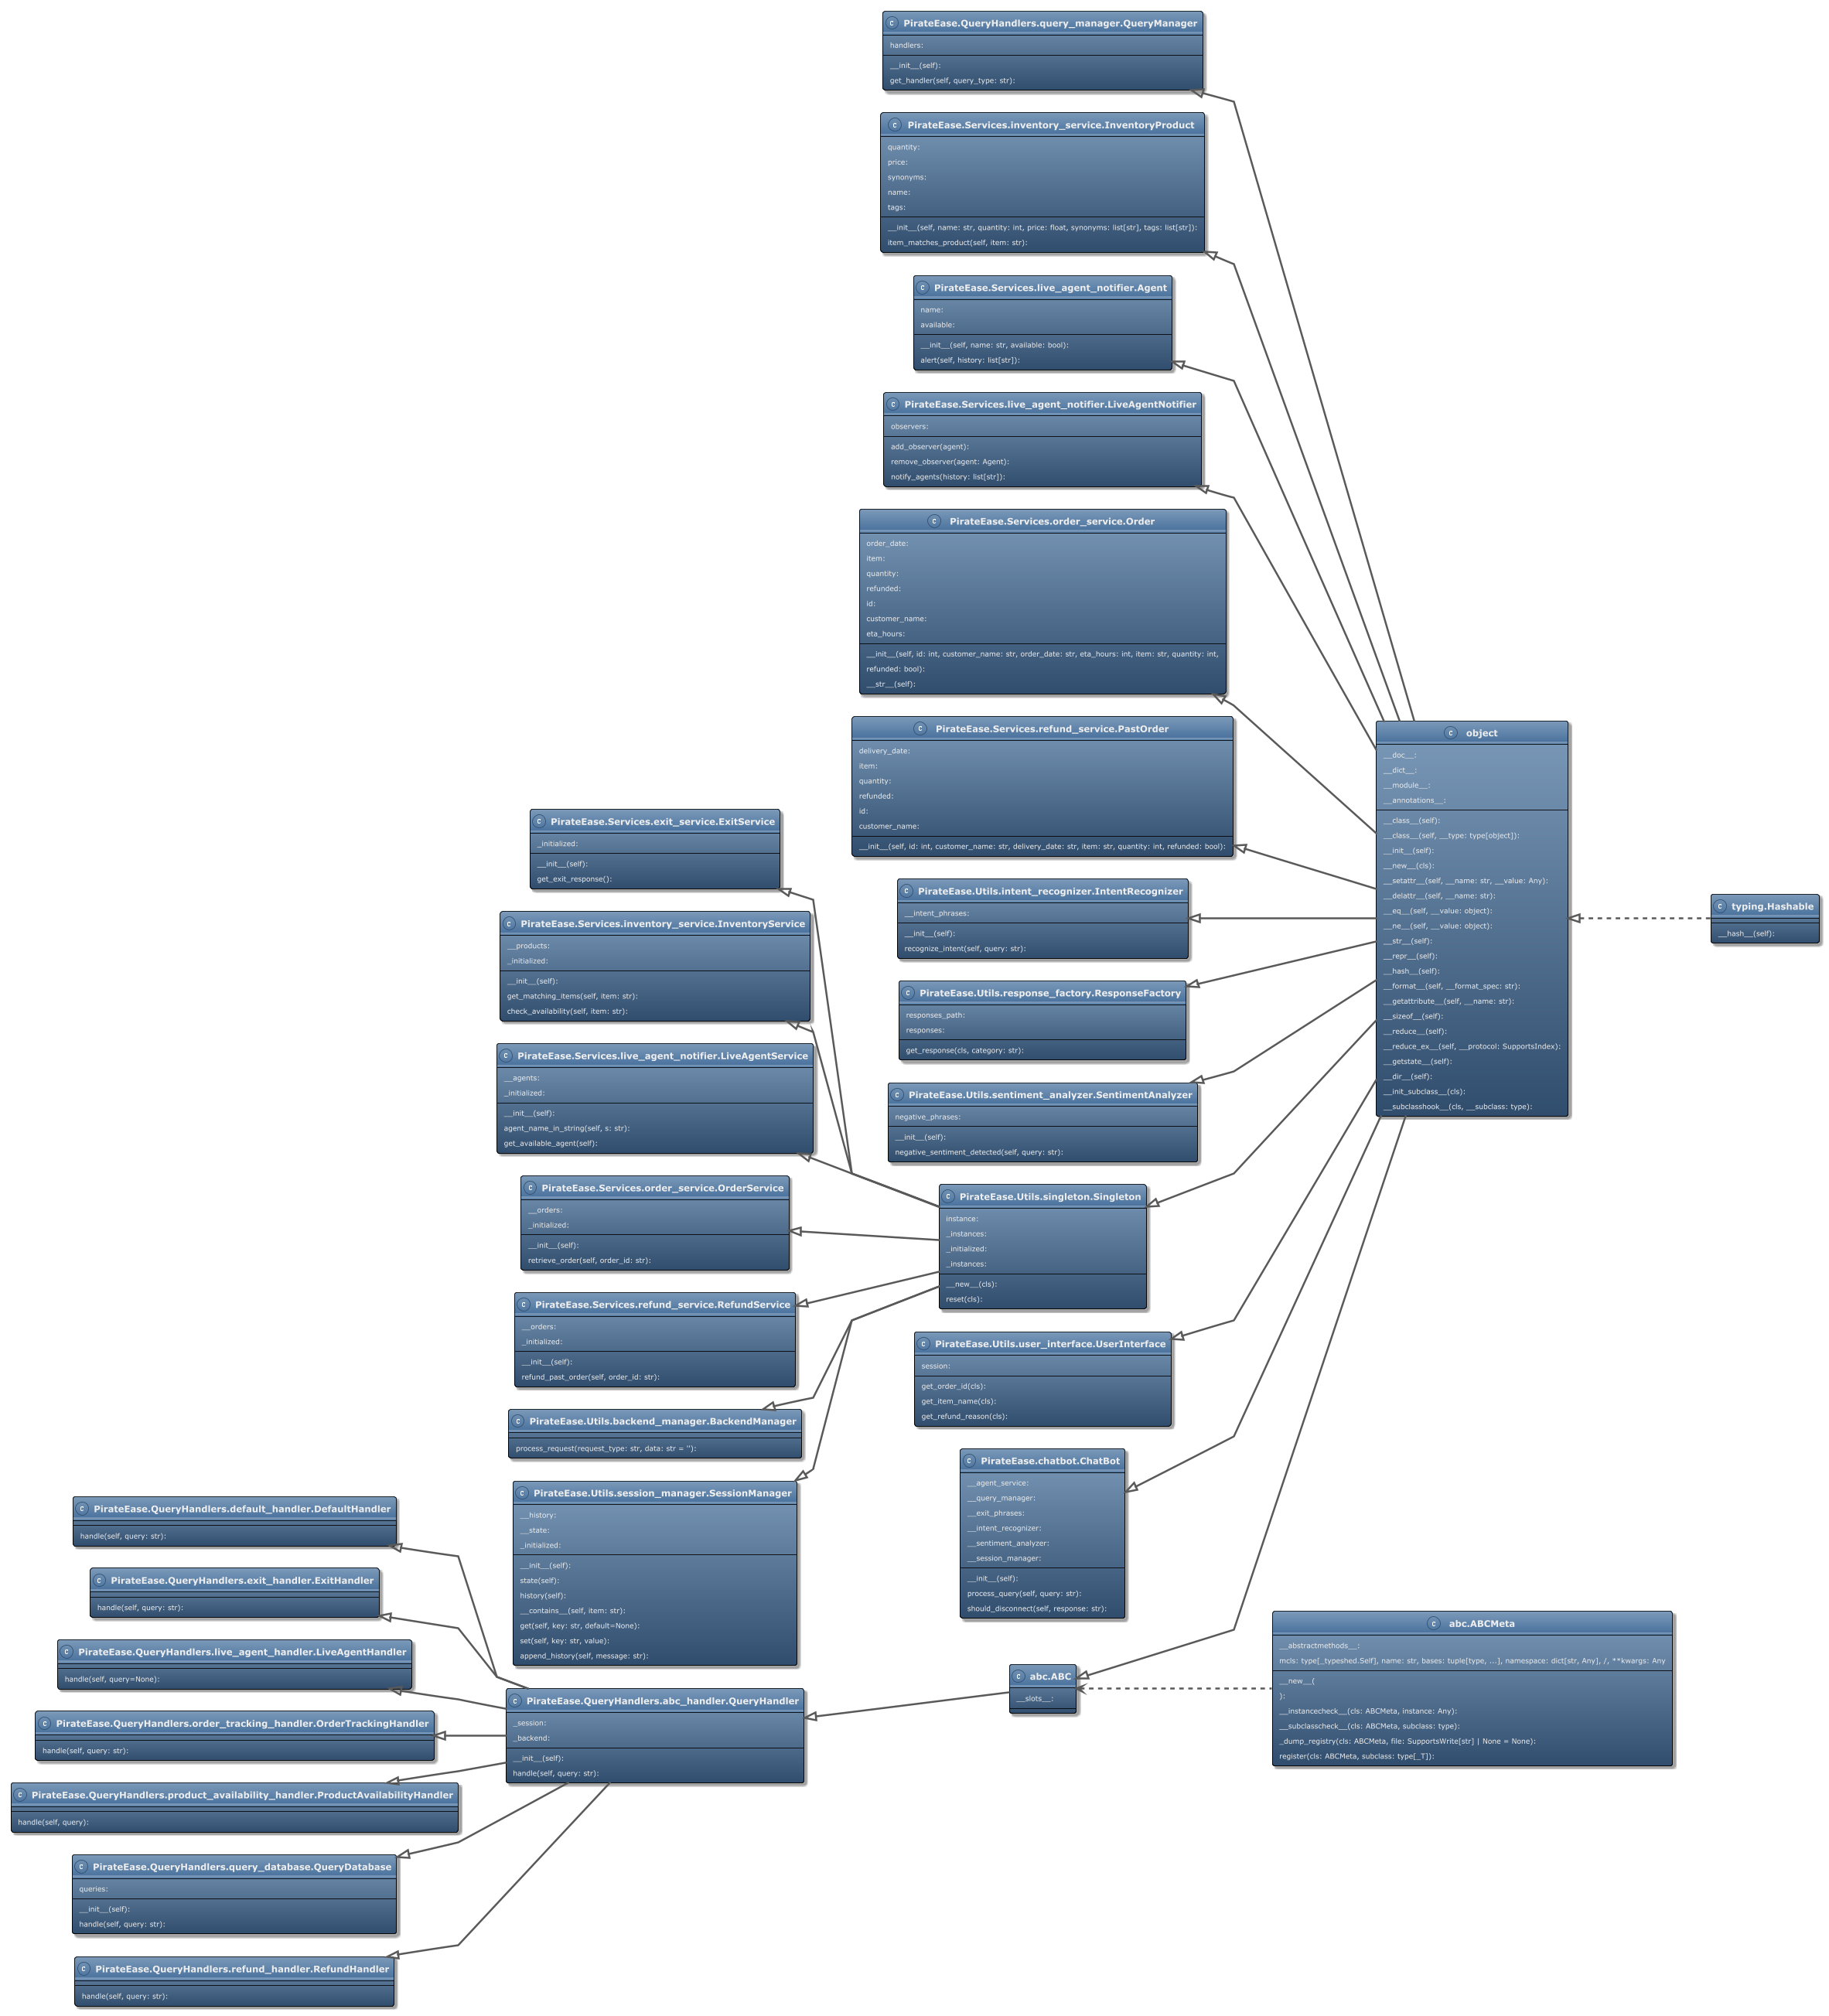
\includegraphics[width=0.8\textwidth,height=0.89\textheight]{diagram.png}
    \caption{UML Class Diagram}
\end{figure}
\noindent
Starting from the right side of the architecture diagram, several classes inherit from the \texttt{Hashable} interface. These classes are organized into clear, logical categories:

\begin{itemize}
	\item \textbf{Data Storage Objects}
		\begin{itemize}
			\item \texttt{InventoryProduct}
			\item \texttt{Agent}
			\item \texttt{Order}
			\item \texttt{PastOrder}
		\end{itemize}

	\item \textbf{Utility Classes}
		\begin{itemize}
			\item \texttt{IntentRecognizer}
			\item \texttt{ResponseFactory}
			\item \texttt{SentimentAnalyzer}
			\item \texttt{Singleton}
			\item \texttt{UserInterface}
		\end{itemize}

	\item \textbf{Notifier}
		\begin{itemize}
			\item \texttt{LiveAgentNotifier}
		\end{itemize}

	\item \textbf{Chatbot Core}
		\begin{itemize}
			\item \texttt{ChatBot}
		\end{itemize}
\end{itemize}
\noindent
Additionally, the following classes explicitly implement the \texttt{Singleton} pattern:
\begin{itemize}
	\item \texttt{ExitService}
	\item \texttt{InventoryService}
	\item \texttt{LiveAgentService}
	\item \texttt{OrderService}
	\item \texttt{RefundService}
	\item \texttt{BackendManager}
	\item \texttt{SessionManager}
\end{itemize}
\noindent
Finally, the query-handling logic is encapsulated within distinct \texttt{QueryHandler} implementations, each derived from the abstract \texttt{QueryHandler} interface:

\begin{itemize}
	\item \texttt{DefaultHandler}
	\item \texttt{ExitHandler}
	\item \texttt{LiveAgentHandler}
	\item \texttt{OrderTrackingHandler}
	\item \texttt{ProductAvailabilityHandler}
	\item \texttt{RefundHandler}
	\item \texttt{QueryDatabase}
\end{itemize}

\newpage

\section{Test Coverage}
\begin{figure}[h!]
    \centering
    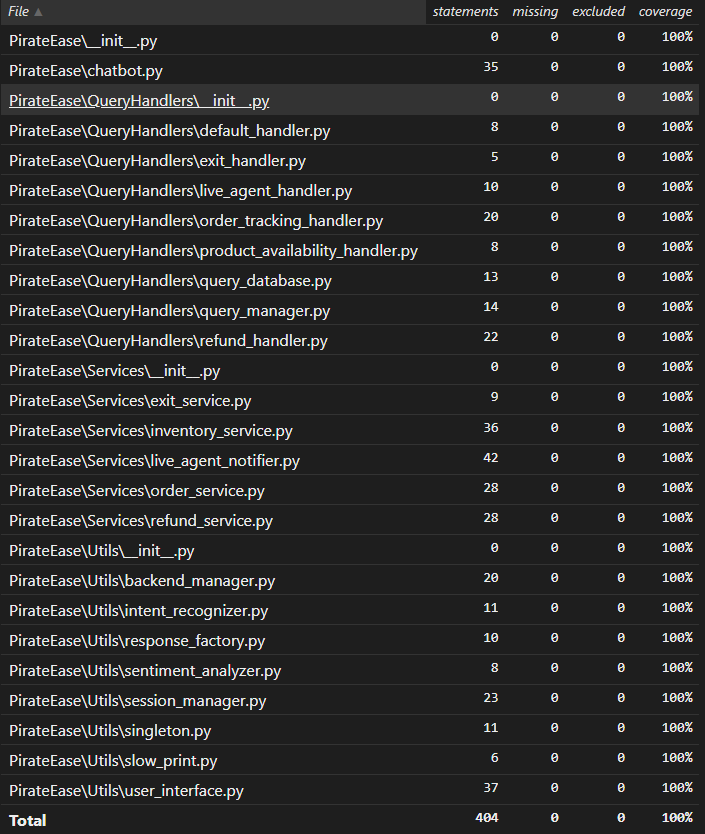
\includegraphics[width=\textwidth]{test_coverage.png}
    \caption{Test Coverage}
\end{figure}	


\section{Screenshots}

\begin{figure}[h!]
    \centering
    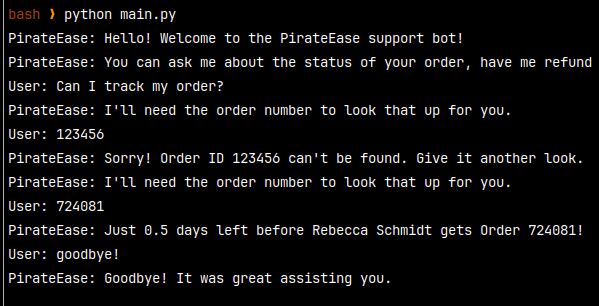
\includegraphics[width=0.8\textwidth]{wrong_then_right_order_id.png}
    \caption{User enters wrong order ID followed by correct order ID}
\end{figure}

\begin{figure}[h!]
    \centering
    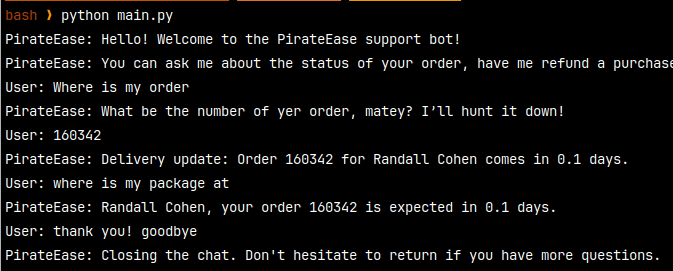
\includegraphics[width=0.8\textwidth]{remembers_order_id.png}
    \caption{Remembers order ID}
\end{figure}

\begin{figure}[h!]
    \centering
    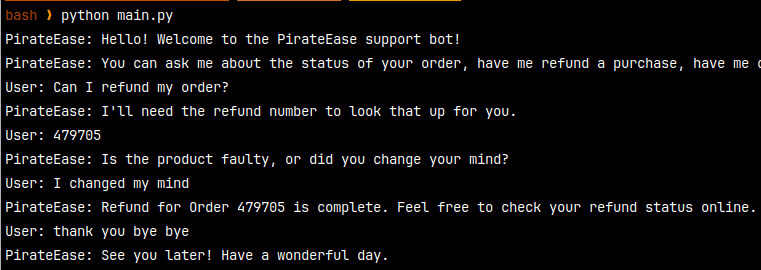
\includegraphics[width=0.8\textwidth]{successful_refund.png}
    \caption{Successful Refund}
\end{figure}

\begin{figure}[h!]
    \centering
    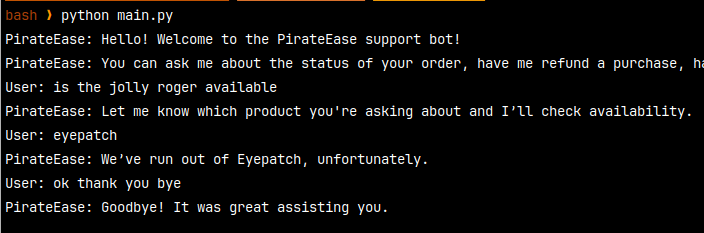
\includegraphics[width=0.8\textwidth]{inventory_out_of_stock.png}
    \caption{Inventory out of Stock}
\end{figure}

\begin{figure}[h!]
    \centering
    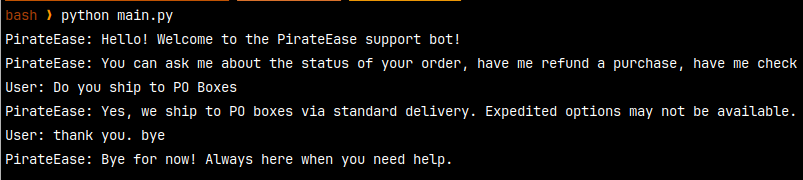
\includegraphics[width=0.8\textwidth]{response_from_database.png}
    \caption{Response from Database}
\end{figure}

\begin{figure}[h!]
    \centering
    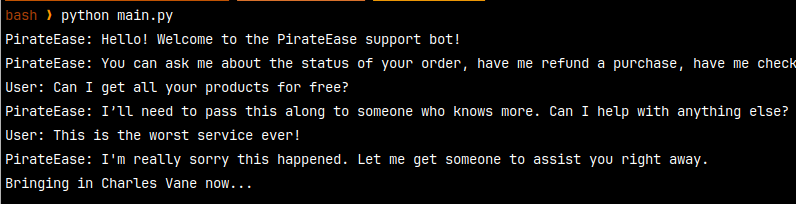
\includegraphics[width=0.8\textwidth]{live_agent_escalation.png}
    \caption{Live Agent Escalation}
\end{figure}



\end{document}